\section{DRAM Structure and Organization}
DRAM-based main memory system is logically organized as a hierarchy of channels, ranks and banks, as illustrated by Figure \ref{fig:dram_org}.
Bank is the smallest structure to be accessed in parallel with each other, which is termed as bank-level parallelism \cite{ISCA08:blp, MICRO09:blp}.
And, rank is formed by clustering multiple, usually eight
\footnote{For illustration purpose, we assume the memory chips are x8, i.e., 8 data I/O pins. The overall structure keeps the same for x4 and x16, except the number of chips in a rank.}
, banks which operate in lockstep, i.e., all banks in a rank respond to a single command. 
Lastly, one channel is composed of an on-chip memory controller and several ranks that share the same narrow command/address and wide data bus.

\begin{figure}
 \centering
  \begin{subfigure}{.34\textwidth}
    \centering
    	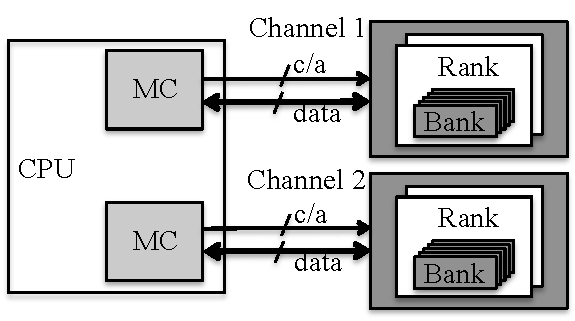
\includegraphics[width=\linewidth]{figures/dram_org.pdf}\\
    \caption{Logical hierarchy}
    \label{fig:dram_org}
  \end{subfigure}
%
  \begin{subfigure}{.39\textwidth}
    \centering
    	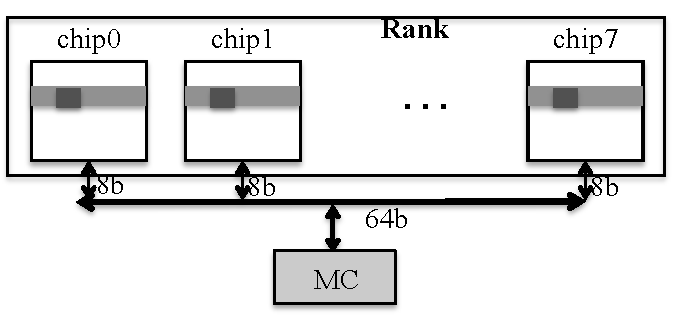
\includegraphics[width=\linewidth]{figures/dram_rank.pdf}\\
    \caption{Rank organization}
    \label{fig:dram_rank}
  \end{subfigure}
  \vspace{-0.45in}
  \caption{DRAM high-level structure.}
  \label{fig:dram}
\end{figure}

Physically, a DRAM rank is composed of multiple chips, inside which eight banks are deployed as cell arrays.
The logical bank, as shown in Figure \ref{fig:dram_org}, is physically made up of the same numbered bank from all chips.
For instance, {\tt bank 0} of a rank contains {\tt bank 0} 
\footnote{Without specific comment in the rest of the thesis, {\tt bank} refers to a logical bank, which is across chips in a rank; for banks residing in a chip, we would specifically call as \ul{chip bank} to differentiate. The same rule goes with {\tt row}.}
residing in all chips in the rank. 
Likewise, a DRAM row is dispersed across chips, as shown in Figure \ref{fig:dram_rank}. 
In normal accesses to a rank, each chip provides 8 bits at a time simultaneously, which together satisfy the total data bus width of 64-bit.
In addition, to amortize memory access overhead on processor side and also to bridge the giant gap between DRAM core frequency (about 200 MHz) and bus frequency (over 1000 MHz), n-bit prefetch and burst access is supported \cite{ISCA11:agms, ISCA14:half_dram}. n is 8 for commodity DDR3, which translates into a granularity of 64B (64b$\times$8), the popular cache block size. 

\begin{figure}
 \centering
  \begin{subfigure}{.36\textwidth}
    \centering
    	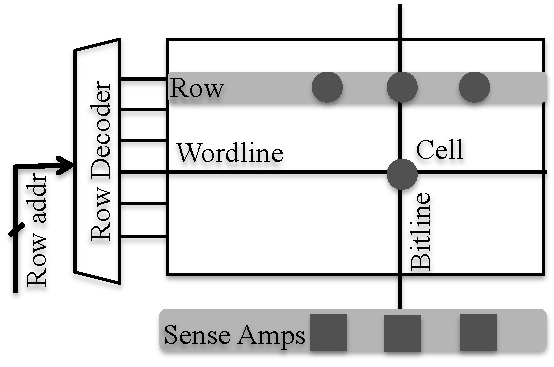
\includegraphics[width=\linewidth]{figures/dram_array.pdf}\\
    \caption{Array}
    \label{fig:dram_array}
  \end{subfigure}
%
  \begin{subfigure}{.16\textwidth}
    \centering
    	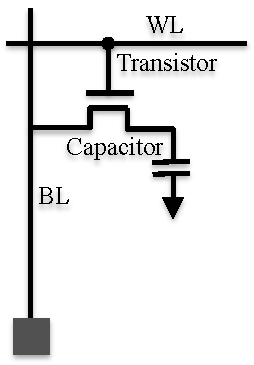
\includegraphics[width=\linewidth]{figures/dram_cell.pdf}\\
    \caption{Cell}
    \label{fig:dram_cell}
  \end{subfigure}
  %
  \begin{subfigure}{.16\textwidth}
    \centering
    	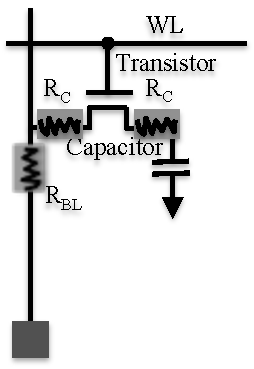
\includegraphics[width=\linewidth]{figures/dram_rc.pdf}\\
    \caption{Circuit}
    \label{fig:dram_rc}
  \end{subfigure}
  \vspace{-0.45in}
  \caption{DRAM detailed organization. (a) is the high-level structure of DRAM array, (b) shows cell structure and (c) illustrates the equivalent circuit where $R_c$ is contact resistance and $R_{BL}$ is the bitline resistance.}
  \label{fig:dram_bank}
  \vspace{-0.45in}
\end{figure}

In more detailed level, DRAM cells are packed into 2D arrays, as Figure \ref{fig:dram_cell} shows, where each cell can be uniquely located by vertically bitline and horizontally wordline.
Each cell consists a capacitor to store electrical charge, and one access transistor to control the connection to wordline.
Upon receiving a row address, DRAM fetches the target row into the row buffer, which contains thousands of sense amplifiers to detect the voltage change on bitline.


\section{DRAM Operations and Timing Constraints}
DRAM supports three types of accesses --- read, write, and refresh. An on-chip memory controller (MC) is responsible to receive requests from processors and decompose them into a series of commands such as {\tt ACT}, {\tt RD}, {\tt WR} and {\tt REF}, etc.
The commands are then sent to DRAM modules sequentially following the predefined timing constraints in DDRx standard. 
We briefly summarize the involved commands and timing constraints as follow: 
%A more comprehensive discussion can be found in \cite{Bruce:Jacob}.

\textbf{READ:} as illustrated in Figure \ref{fig:dram_read}, read access starts with an \underline{ACTIVATE} (ACT) command to bring the required row into the sense amplifiers; then, a \underline{READ} (RD) command is issued to fetch data from the row buffer. The interval between  ACT and RD is constrained by {\tt tRCD}. DRAM read is destructive, and hence the charge in the storage capacitors needs to be restored. The restore operation is performed concurrently with RD, and a row cannot be closed until restoring completes, which is determined by {\tt tRAS-tRCD}. Once the row is closed, a \underline{PRECHARGE} (PRE) can be issued to prepare for a new row access. PRE is constrained by timing {\tt tRP}. The time for the whole read process is {\tt tRC=tRAS+tRP}.

\begin{figure}
 \centering
  \begin{subfigure}{.7\textwidth}
    \centering
    	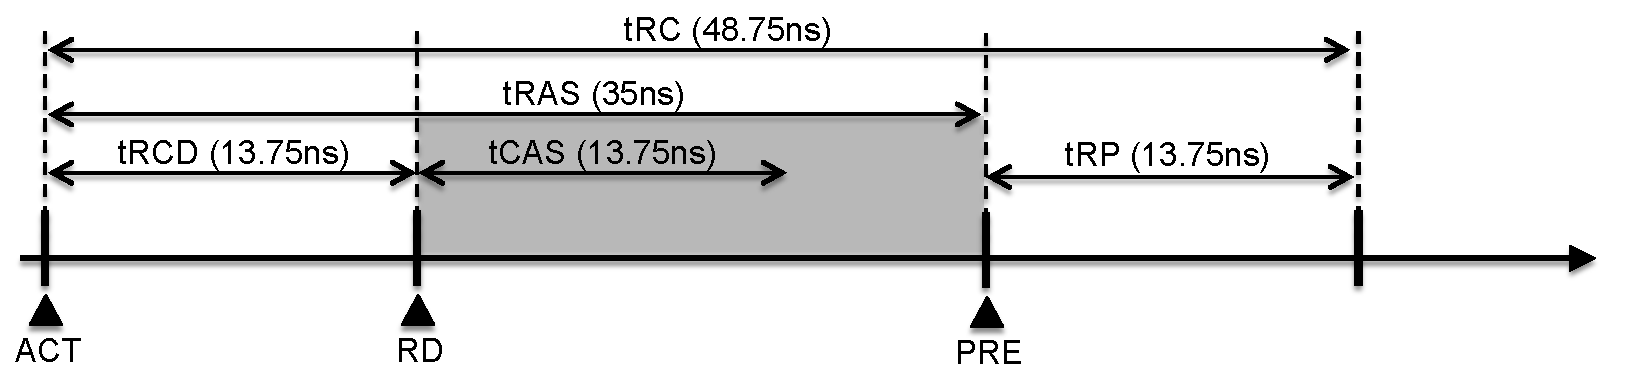
\includegraphics[width=\linewidth]{figures/timing_read.pdf}\\
    \caption{Read operation}
    \label{fig:dram_read}
  \end{subfigure}

\vspace{-0.25in}
  \begin{subfigure}{.7\textwidth}
    \centering
    	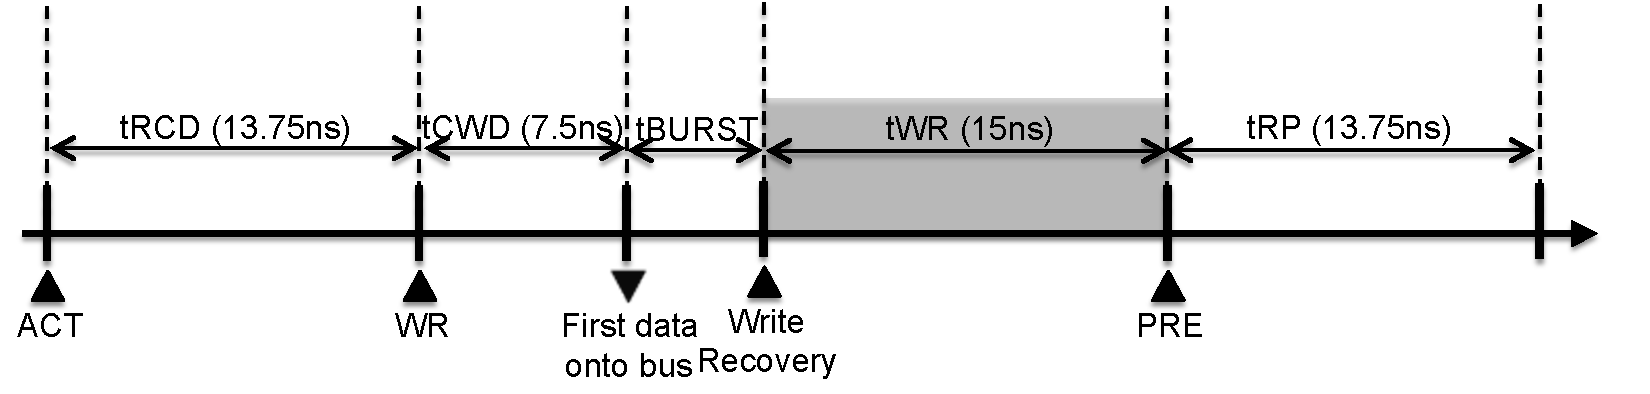
\includegraphics[width=\linewidth]{figures/timing_write.pdf}\\
    \caption{Write operation}
    \label{fig:dram_write}
  \end{subfigure}
  \vspace{-0.4in}
  \caption{Commands and timing constraints involved in DRAM accesses. (Timing values are from  \cite{JEDEC:ddr3})}
  \label{fig:operation}
    \vspace{-0.45in}
\end{figure}

\textbf{WRITE:} write works similarly to read, with ACT as the first command to be performed. After {\tt tRCD} has been elapsed, a \underline{WRITE} (WR) is issued to overwrite the content in the row buffer, and then update (restore) the value back into the DRAM cells. Before issuing PRE, the new data overwritten in the sense amps must be safely restored into the target bank, taking {\tt tWR} time. 
To summarize, both RD and WR commands involve the restoring operation
\footnote{Whereas restoring after write is represented by {\tt tWR}, that after read is included in {\tt tRAS}. For ease of presentation, we discuss with a focus on {\tt tWR} and always adjust {\tt tRAS} accordingly.}
, and hence a change in restore time shall affect both DRAM read and write accesses. 

\textbf{Refresh:}
%DRAM needs to be refreshed periodically to prevent data loss. 
refresh commands are issued by memory controller typically every 7.8$\mu$s to refresh a bin, which is composed of multiple rows.
Upon receiving {\tt REF}, DRAM device refresh the designated rows tracked by the internal counter.
%According to JEDEC \cite{JEDEC:ddr3}, 8192 all-bank auto-refresh ({\tt REF}) commands are sent to all DRAM devices in a rank within one retention time interval ({\tt Tret}), also called as one refresh window ({\tt tREFW}) \cite{TC15:refresh, ISCA13:ddr4, HPCA14:parallelrefresh}, typically 64ms for DDR3/4. 
%The gap between two {\tt REF} commands is termed as refresh interval ({\tt tREFI}), whose typical value is 7.8$\mu$s, i.e. 64ms/8192.
%If a DRAM device has more than 8192 rows, rows are grouped into 8192 {\bf refresh bins}. One {\tt REF} command is used to refresh multiple rows in a bin. An internal counter in each DRAM device tracks the designated rows to be refreshed upon receiving {\tt REF}. 
The refresh operation takes {\tt tRFC} to complete, which proportionally depends on the number of rows in the bin.
Whereas typically the whole memory rank is refreshed every 64ms, the vast majority cells can hold data for a much longer time \cite{ISCA12:raidr, ISCA15:reflex}.

\section{DRAM Technology Scaling}
\subsection{Scaling Issues}
With continuously increasing demands on DRAM density and capacity, the cell dimensions keep scaling downward.
%Memory technology scaling drives increasing density and capacity by decreasing cell dimensions.
Past decades saw DRAM's rapid development of 4x density every 3 years \cite{BOOK:cod}. 
Along scaling path from over 100nm to nowadays 2x nm, DRAM also experiences the drop of supply voltage \cite{HPCA16:twr}, more severe signal noise \cite{ISQED08:offset, ISCA13:ddr4} and shorter retention time \cite{ISCA13:archshield, PATENT15:twr}.
However, for reliable operations in DRAM, cell capacitor must be sufficiently large to hold sufficient charge, access transistor is required to be large enough to exert effective control \cite{ISCA09:pcm}, resistance should not be too large to obstruct cell charging process, and sub-threshold leakage should be small to safely hold data for a long time.

The intertwining requirements make the scaling jeopardy. For instance, smaller technology nodes provides smaller contacts of transistor and capacitor, and also narrower bitlines, both of which result in increased resistance (shown in Figure \ref{fig:dram_rc}), which lengthens the restoring time, and further the overall access latency. The growing number of slow and leaky cells has a large impact on system performance. 
There are three general strategies to address this challenge:
\begin{itemize}
\itemsep -1pt
\item 
The first choice is to keep conventional hard timing constraints for DRAM, 
which makes it challenging to handle slow and leaky cells.  Cells that fall
outside of guardbands could be filtered (not used).
% when they are outside guardbands.  
With scaling, however, this approach can incur worse chip yield
and higher manufacturing cost. 
%One choice is not to expose these cells by filtering out chips with weak cells above a threshold. This results in low chip yield and high manufacturing cost. 
Because the DRAM industry operates in an environment of exceedingly tight profit
margins, reducing chip yield for commodity devices is unlikely to be preferred.
%Given that DRAM industry is known for its tight profit margin, reducing chip yield may not be preferred. 

\item 
A second choice is to expose weak cells, falling outside guardbands, and integrate strong yet complex error correction schemes, e.g., \textit{ArchShield} \cite{ISCA13:archshield}. Due to the large number of cells that violate conventional timing constraints such as {\tt tRCD}, {\tt tWR}, significant space and performance overheads are expected.

\item
A third choice is to relax timing constraints \cite{MEM14:twr, DATE15:twr}. This approach is compelling because it can easily maintain high chip yield at extreme technology sizes. 
%Studies suggested relaxed timing constraints in future DRAM chips \cite{MEM14:twr, DATE15:twr}, which helps to keep high yield to make the technology viable. 
However, relaxing timing, without careful management, can cause 
large performance penalties.  
\end{itemize} 
%
Because the third choice is compatible with the need for high chip density 
and yield, we adopt it in this thesis.  We relax restore timing and strive to mitigate associated 
performance degradation. 
Our design principle is also applicable to the second strategy if exposed errors 
can be well managed. We leave this possibility to future work.

\subsection{Related Work on Restoring}
While write recovery time ({\tt tWR}) keeps at 15ns across all generations from DDR to DDR4 \cite{JEDEC:ddr, JEDEC:ddr2, JEDEC:ddr3, JEDEC:ddr4}, it has to be lengthened in deep sub-micron technology nodes, which was first recently discussed by \citeN{MEM14:twr}.
As the first academic work on {\tt tWR} issues in further scaling DRAM, our paper \cite{DATE15:twr} studied the variation behaviors and proposed to utilize chunk remapping to lower restoration durations.
Afterwards, patents on {\tt tWR} were granted: \citeN{PATENT14:twr} raised the idea to adjust timings with respect to temperature, and \citeN{PATENT15:twr} claimed that {\tt tWR} can be increased from 15ns to 60ns, and then raised the idea of exploring backward compatibility.

Whereas the {\tt tWR} scaling issue has been identified in industrials, little academic research have been performed. Restoration has been an silent issue util recently; people started to utilize the reserved timing margins \cite{DATE14:margin, HPCA15:al-dram}, with restoring being included. Besides, later work \cite{ISCA15:mcr} took use of charge variation to relax some timing constraints. However, none of these work targets at future DRAM technologies.

%\section{Related Work}